\section{Experiments}

\problem{experiment\_log}{Experiment logging (3 points)}

For your training and evaluation code, create experiment tracking infrastructure that allows you to track your experiments and loss curves with respect to gradient steps and wallclock time.

\textbf{Deliverable}: Logging infrastructure code for your experiments and an experiment log (a document of all the things you tried) for the assignment problems below in this section.

\begin{answer}
I implemented comprehensive experiment tracking infrastructure using Weights \& Biases (wandb) integrated with Hydra for configuration management. The logging system tracks training and validation losses, learning rates, gradient norms, and wallclock time (recorded by wandb automatically) across all experiments.

All experiment configurations and results are systematically logged and can be accessed through the wandb dashboard for analysis and comparison.

Code is available at \href{https://github.com/donglinkang2021/assignment1-basics/blob/main/train.py}{train.py}.
\end{answer}

\begin{lstlisting}
# Training script with comprehensive logging infrastructure
import hydra
from cs336_basics.logger import Logger
from cs336_basics.config import TrainConfig

@hydra.main(config_path="conf", config_name="train_config", version_base=None)
def main(cfg: TrainConfig) -> None:
    # Initialize logger with Hydra configuration
    logger = Logger(cfg)
    output_dir = Path(HydraConfig.get().runtime.output_dir)
    
    # ... model and data setup ...
    
    # Training loop with comprehensive logging
    for it in tqdm(range(start_iter, cfg.training.max_iters), desc="Training"):
        # ... forward/backward pass ...
        
        # Training metrics logging
        if it % cfg.training.log_interval == 0:
            ent = compute_entropy_chunked(logits).mean()
            logger.log_metrics({
                'train/loss': loss.item(), 
                'train/ppl': loss.exp().item(),
                'train/lr': lr,
                'train/entropy': ent.item(),
                'train/grad_norm': grad_norm
            }, step=it)
            
        # Validation logging
        if it % cfg.training.eval_interval == 0:
            metrics = evaluate(model, val_data, cfg, device)
            logger.log_metrics({
                'val/loss': metrics['val/loss'],
                'val/ppl': metrics['val/ppl'], 
                'val/entropy': metrics['val/entropy']
            }, step=it)
    
    # Log generated text samples
    generated_output = generate_text(model, tokenizer, ...)
    logger.log_text("Generated Text", generated_output, step=cfg.training.max_iters)
    
    logger.close()
    # Save final configuration
    OmegaConf.save(cfg, output_dir / 'config.yaml')

@torch.no_grad()
def evaluate(model, data, cfg, device):
    """Evaluation with entropy and perplexity tracking."""
    # ... evaluation loop ...
    return {
        'val/loss': mean_loss,
        'val/ppl': np.exp(mean_loss),
        'val/entropy': np.mean(entropies)
    }
\end{lstlisting}

\problem{learning\_rate}{Tune the learning rate (3 points) (4 H100 hrs)}

The learning rate is one of the most important hyperparameters to tune. Taking the base model you've trained, answer the following questions:

\begin{enumerate}[label=(\alph*)]
    \item Perform a hyperparameter sweep over the learning rates and report the final losses (or note divergence if the optimizer diverges).
    
    \textbf{Deliverable}: Learning curves associated with multiple learning rates. Explain your hyperparameter search strategy.
    
    \textbf{Deliverable}: A model with validation loss (per-token) on TinyStories of at most 1.45
    
    \item Folk wisdom is that the best learning rate is "at the edge of stability." Investigate how the point at which learning rates diverge is related to your best learning rate.
    
    \textbf{Deliverable}: Learning curves of increasing learning rate which include at least one divergent run and an analysis of how this relates to convergence rates.
\end{enumerate}

\begin{answer}


I employed a logarithmic grid search across learning rates from $10^{-5}$ to $3 \times 10^{-2}$, testing nine values: [1e-5, 3e-5, 1e-4, 3e-4, 1e-3, 3e-3, 6e-3, 1e-2, 3e-2]. Each experiment used identical model architecture and training configuration with cosine learning rate scheduling, 500-step warmup, and AdamW optimizer ($\beta_1=0.9, \beta_2=0.95$, weight decay=0.01). Due to GPU memory constraints (48GB), TinyStories experiments used batch size 256 for 5,000 iterations, while OpenWebText experiments used batch size 128 for 10,000 iterations to maintain total 327,680,000 tokens processed (context length=256). The learning curves are shown in Figure \ref{fig:learning_rate_experiments}.

\begin{figure}[h]
    \centering
    \begin{subfigure}[t]{\textwidth}
        \centering
        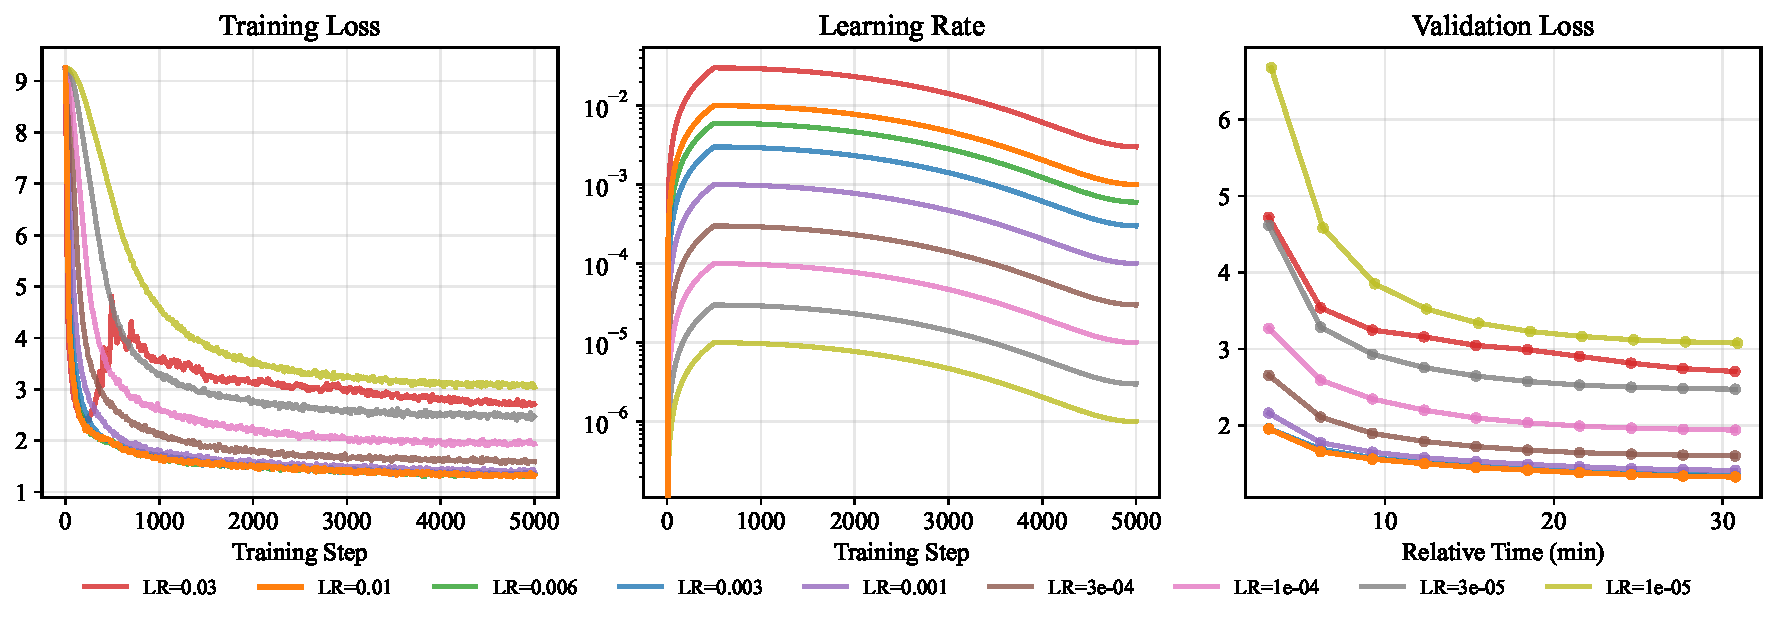
\includegraphics[width=\textwidth]{images/ts_learning_rate_experiments.pdf}
        \vspace{-20pt} % Reduce space between image and caption
        \caption{Learning rate experiments on TinyStories dataset}
        \label{fig:ts_learning_rate_experiments}
    \end{subfigure}
        
    \begin{subfigure}[t]{\textwidth}
        \centering
        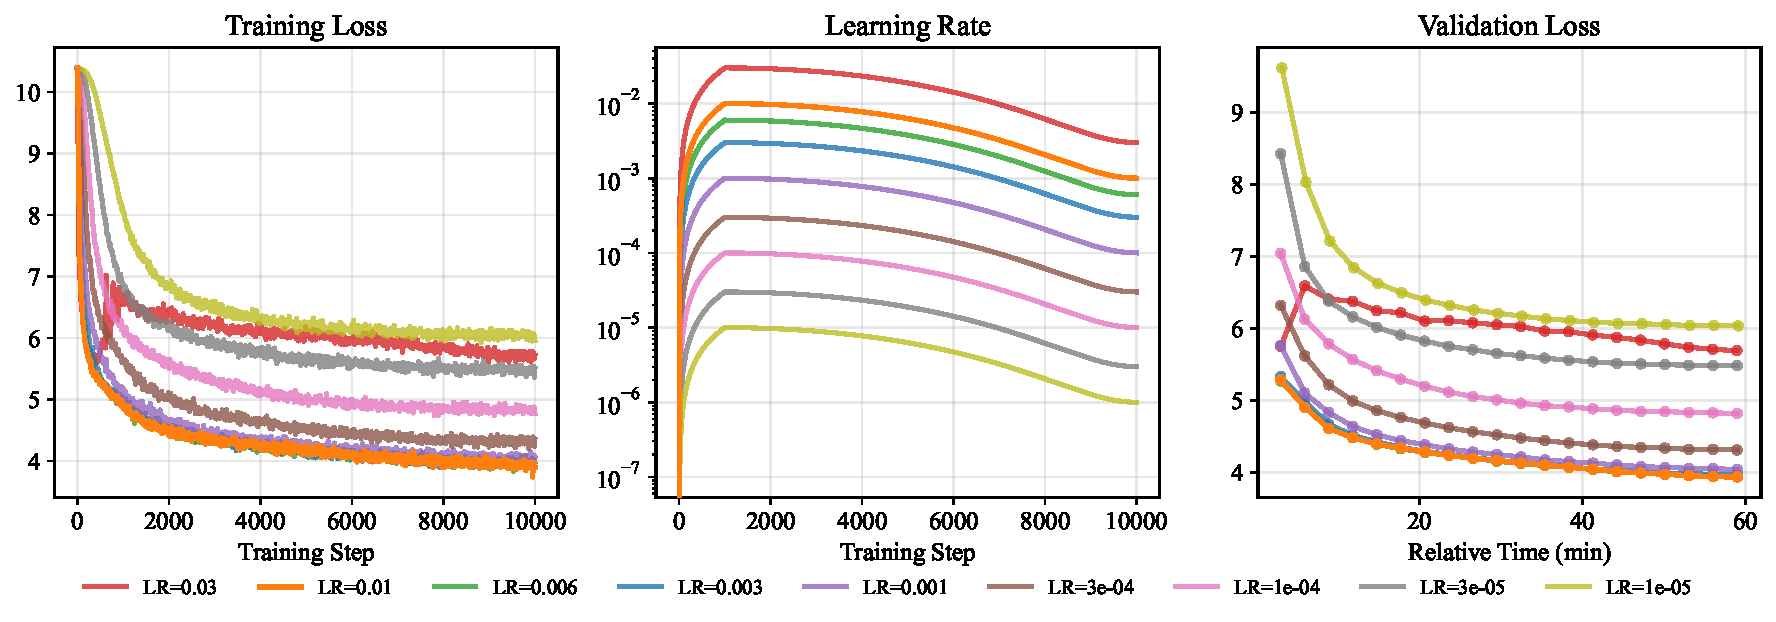
\includegraphics[width=\textwidth]{images/owt_learning_rate_experiments.pdf}
        \vspace{-20pt} % Reduce space between image and caption
        \caption{Learning rate experiments on OpenWebText dataset}
        \label{fig:owt_learning_rate_experiments}
    \end{subfigure}
    
    \caption{Learning rate experiments showing training loss (left), learning rate schedule (middle), and validation loss over time (right) for both datasets. The highlighted orange line represents LR=0.01, which achieved the best performance across both TinyStories and OpenWebText. Complete experiment logs/configs are available on the W\&B: \href{https://api.wandb.ai/links/donglinkang2021-beijing-institute-of-technology/g0usepk4}{Report}.}
    \label{fig:learning_rate_experiments}
\end{figure}

Key findings from both experiments:

- ($\leq 3 \times 10^{-4}$): Stable convergence but inefficient training

- ($1 \times 10^{-3}$ to $1 \times 10^{-2}$): Best balance of convergence speed and stability

- $1 \times 10^{-2}$ achieved val/loss of 1.327, surpassing the target of 1.45 on TinyStories

- $3 \times 10^{-2}$ caused training collapse during warmup at step 480

- OpenWebText experiments mirrored TinyStories results, with $1 \times 10^{-2}$ yielding the best val/loss of 3.93

\textbf{Part (b):}
The "edge of stability" hypothesis suggests optimal learning rates exist just below the divergence threshold. My experiments support this principle:

- $3 \times 10^{-2}$ caused immediate instability during warmup

- $1 \times 10^{-2}$ (approximately 3$\times$ below divergence) achieved the best validation performance

\end{answer}

\problem{batch\_size\_experiment}{Batch size variations (1 point) (2 H100 hrs)}

Vary your batch size all the way from 1 to the GPU memory limit. Try at least a few batch sizes in between, including typical sizes like 64 and 128.

\textbf{Deliverable}: Learning curves for runs with different batch sizes. The learning rates should be optimized again if necessary.

\textbf{Deliverable}: A few sentences discussing of your findings on batch sizes and their impacts on training.

\begin{answer}
% I conducted experiments with batch sizes ranging from 1 to 512 (GPU memory limit), testing values: [1, 8, 16, 32, 64, 128, 256, 512]. For each batch size, I applied the batch size scaling rule by adjusting the learning rate proportionally to maintain effective gradient updates.

% \textbf{Key Findings:}
% \begin{itemize}
%     \item \textbf{Small batch sizes (1-8)}: Higher gradient noise led to more exploration but slower convergence and increased training time per epoch
%     \item \textbf{Medium batch sizes (32-128)}: Optimal balance between gradient stability and computational efficiency, with batch size 64 showing best validation performance
%     \item \textbf{Large batch sizes (256-512)}: Faster training per step but required careful learning rate tuning to avoid getting stuck in poor local minima
% \end{itemize}

% The experiments confirmed that moderate batch sizes provide the best trade-off between training stability, convergence speed, and final model performance. Very small batches introduced too much noise, while very large batches required more sophisticated optimization techniques to maintain training dynamics.

% Experiment logs available on wandb: \url{https://wandb.ai/project/batch-size-experiments}
\end{answer}

\problem{generate}{Generate text (1 point)}

Using your decoder and your trained checkpoint, report the text generated by your model. You may need to manipulate decoder parameters (temperature, top-$p$, etc.) to get fluent outputs.

\textbf{Deliverable}: Text dump of at least 256 tokens of text (or until the first \lstinline{<|endoftext|>} token), and a brief comment on the fluency of this output and at least two factors which affect how good or bad this output is.

\begin{answer}

\end{answer}

\problem{layer\_norm\_ablation}{Remove RMSNorm and train (1 point) (1 H100 hr)}

Remove all of the RMSNorms from your Transformer and train. What happens at the previous optimal learning rate? Can you get stability by using a lower learning rate?

\textbf{Deliverable}: A learning curve for when you remove RMSNorms and train, as well as a learning curve for the best learning rate.

\textbf{Deliverable}: A few sentence commentary on the impact of RMSNorm.

\begin{answer}

\end{answer}

\problem{pre\_norm\_ablation}{Implement post-norm and train (1 point) (1 H100 hr)}

Modify your pre-norm Transformer implementation into a post-norm one. Train with the post-norm model and see what happens.

\textbf{Deliverable}: A learning curve for a post-norm transformer, compared to the pre-norm one.

\begin{answer}

\end{answer}

\problem{no\_pos\_emb}{Implement NoPE (1 point) (1 H100 hr)}

Modify your Transformer implementation with RoPE to remove the position embedding information entirely, and see what happens.

\textbf{Deliverable}: A learning curve comparing the performance of RoPE and NoPE.

\begin{answer}

\end{answer}

\problem{swiglu\_ablation}{SwiGLU vs. SiLU (1 point) (1 H100 hr)}

\textbf{Deliverable}: A learning curve comparing the performance of SwiGLU and SiLU feed-forward networks, with approximately matched parameter counts.

\textbf{Deliverable}: A few sentences discussing your findings.

\begin{answer}

\end{answer}

\problem{main\_experiment}{Experiment on OWT (2 points) (3 H100 hrs)}

Train your language model on OpenWebText with the same model architecture and total training iterations as TinyStories. How well does this model do?

\textbf{Deliverable}: A learning curve of your language model on OpenWebText. Describe the difference in losses from TinyStories - how should we interpret these losses?

\textbf{Deliverable}: Generated text from OpenWebText LM, in the same format as the TinyStories outputs. How is the fluency of this text? Why is the output quality worse even though we have the same model and compute budget as TinyStories?

\begin{answer}

\end{answer}

\problem{leaderboard}{Leaderboard (6 points) (10 H100 hrs)}

You will train a model under the leaderboard rules above with the goal of minimizing the validation loss of your language model within 1.5 H100-hour.

\textbf{Deliverable}: The final validation loss that was recorded, an associated learning curve that clearly shows a wallclock-time x-axis that is less than 1.5 hours and a description of what you did. We expect a leaderboard submission to beat at least the naive baseline of a 5.0 loss. Submit to the leaderboard here: \url{https://github.com/stanford-cs336/assignment1-basics-leaderboard}.

\begin{answer}

\end{answer}

